\documentclass[a4paper]{article}
\usepackage{graphicx} % Required for inserting images
\usepackage{amssymb}
\usepackage{amsmath}
\usepackage{hyperref}
\usepackage{listings}
\usepackage{fancyhdr}
\usepackage{xcolor}
\usepackage{geometry}
\usepackage{ragged2e}
\usepackage{subcaption}
\usepackage{multirow}
\usepackage{tabularx}
\usepackage{indentfirst}
\usepackage{lscape}
\usepackage{titlesec}
\usepackage[nottoc,numbib]{tocbibind}
\usepackage[usenames, dvipsnames]{xcolor}
\usepackage{tikz} \usetikzlibrary{calc}


\geometry{margin=1in}

\colorlet{myGreen}{green!70!black}
\colorlet{myDGreen}{green!50!black}
\colorlet{myGray}{white!60!black}

\newcommand{\colNaN}[1]{{\textcolor{black!30}{#1}}}
\newcommand{\colDisaster}[1]{{\textcolor{red!60}{#1}}}
\newcommand{\colFailure}[1]{{\textcolor{orange}{#1}}}
\newcommand{\colWorse}[1]{\textcolor{orange!60}{#1}}
\newcommand{\colSimilar}[1]{\textcolor{black!60}{#1}}
\newcommand{\colBetter}[1]{\textcolor{blue!70}{#1}}
\newcommand{\colSuccess}[1]{\textcolor{black!30!green}{#1}}
\newcommand{\colAmazing}[1]{\textcolor{green}{#1}}

\hypersetup{
    colorlinks,
    linkcolor={blue!50!black},
    citecolor={blue!50!black},
    urlcolor={blue!80!black}
}

\lstdefinestyle{mystyle}{
    language=Python,
    backgroundcolor=\color{white!95!black},   
    %commentstyle=\color{},
    %keywordstyle=\color{},
    %numberstyle=\tiny\color{codegray},
    %stringstyle=\color{codepurple},
    basicstyle=\ttfamily\footnotesize,
    breakatwhitespace=false,         
    breaklines=true,                 
    %captionpos=b,                    
    keepspaces=true,                 
    %numbers=left,                    
    %numbersep=5pt,                  
    showspaces=false,                
    showstringspaces=false,
    showtabs=false,                  
    tabsize=4,
}
\lstset{
    style=mystyle,
    %emph={sage},
    %emphstyle={\color{myGreen}}
}



%\renewcommand\footnoterule{\rule{.4\textwidth}{0.2pt}}
\renewcommand\footnoterule{\kern-3pt \hrule  \kern 2.6pt}
\fancyhead[L, C]{}
\fancyfoot[C]{\thepage}
\pagestyle{fancy}

\title{Internship report}
\author{Marie BONBOIRE}
\date{}

\begin{document}

\thispagestyle{plain}
\begin{titlepage}
    \begin{figure}[h]
        \centering
        
\includegraphics[width=0.4\textwidth]{su.png}
    \end{figure}
    \vspace{1cm}

    \begin{center}
        {\LARGE PCCA}\\[0.3cm]
        \rule{\linewidth}{0.5mm} \\[0.4cm]
        {\huge \textbf{Arithmétique modulaire et vectorisation\\ SIMD / AVX}}\\[0.4cm]
        \rule{\linewidth}{0.5mm} \\[1cm]
        {\large 24 January 2025 - ?? May 2025}\\[3cm]

        {\Large Damien ASSIRE \& Marie BONBOIRE}


    \end{center}

    \vfill
\begin{flushleft}{\large
    \textbf{Supervisor:} Mr. Vincent NEIGER (LIP6 - PolSys)\\
    }
\end{flushleft}
\end{titlepage}
\newpage

\tableofcontents
\newpage

\section{Preface}

\paragraph{goals}
\begin{itemize}
    \item Implement basic arithemic operations (scalar-vector multiplication, vector-vector multiplication, dot product) using Flint.
    \item Improve these operations using Intel's intrinsics for Single Instruction Multiple Datas (SIMD) vectorization.
    \item Advanced benchmarking/profiling.
    \item Apply on a form of butterfly FFT for a forward integration to Flint.
\end{itemize}




\subsection{Machines description}


% 2023 - 4.5 GHz % mariz
% 2019 - 2.5 GHz % ppti
% 2023 - 3.3 GHz % argiope
% 2021 - 3.0 GHz % groebner

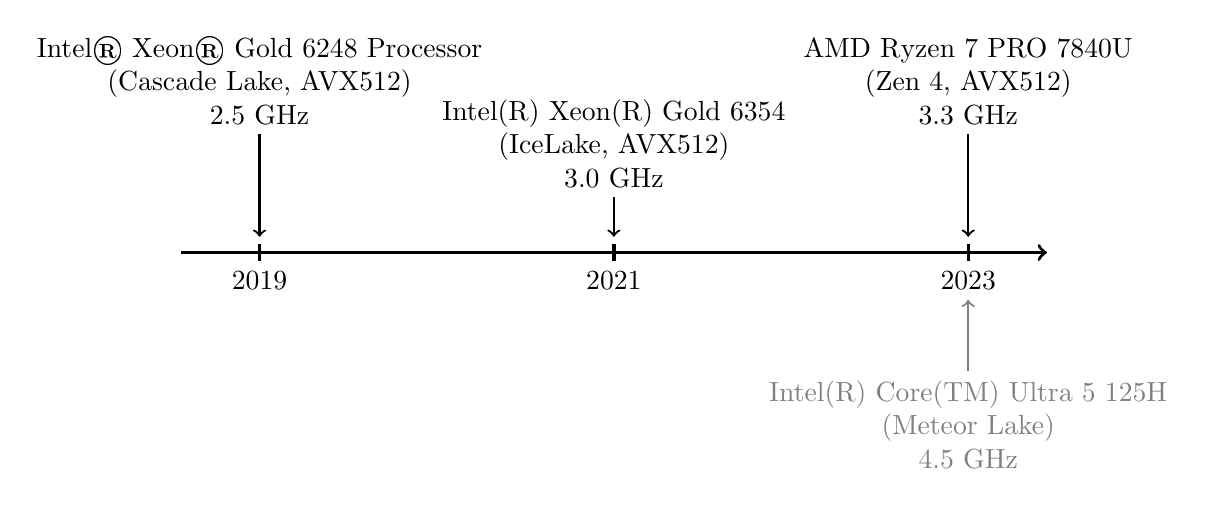
\begin{tikzpicture}[very thick, black]

    %coordinates
    \coordinate (O) at (1,0); % Origin
    \coordinate (F) at (12,0); %End
    \coordinate (P1) at (2,0); %ppti
    \coordinate (P2) at (6.5,0); %groebner
    \coordinate (P3) at (11,0); %mariz+argiope

    %proc
    \draw[<-,thick,color=black] ($(P1)+(0,0.2)$) -- ($(P1)+(0,1.5)$) node [above=0pt,align=center,black] 
    {Intel® Xeon® Gold 6248 Processor \\ (Cascade Lake, AVX512) \\ 2.5 GHz};
    \draw[<-,thick,color=black] ($(P2)+(0,0.2)$) -- ($(P2)+(0,0.7)$) node [above=0pt,align=center,black] 
    {Intel(R) Xeon(R) Gold 6354 \\ (IceLake, AVX512) \\ 3.0 GHz};
    \draw[<-,thick,color=black] ($(P3)+(0,0.2)$) -- ($(P3)+(0,1.5)$) node [above=0pt,align=center,black] 
    {AMD Ryzen 7 PRO 7840U \\ (Zen 4, AVX512) \\ 3.3 GHz};
    \draw[<-,thick,color=gray] ($(P3)-(0,0.6)$) -- ($(P3)-(0,1.5)$) node [below=0pt,align=center,gray] 
    {Intel(R) Core(TM) Ultra 5 125H \\ (Meteor Lake) \\ 4.5 GHz};

    %main arrow
    \draw[->] (O) -- (F);

    %ticks
    \foreach \x in {2,6.5,11}
    \draw(\x cm,3pt) -- (\x cm,-3pt);
    %labels
    \foreach \i \j in {2/2019,6.5/2021,11/2023}{
    	\draw (\i,0) node[below=3pt] {\j} ;
    }

\end{tikzpicture}

\section{Multiplication of 64 bits integers}

When multiplying two integers, a problem of overflow can arise since the result might be too big to be stored in a 64 bits word. 
To circumvent this issue, one needs to first split the two integers into two words of a given size and then apply the long multiplication.

That is, given two integers $a$ and $b$ each of at most 64 bits, we start by splitting them into 2 words of $k$ bits with $k<64$:

\begin{align*}
    a &= a_{hi}\cdot 2^{k} + a_{lo} \\
    b &= b_{hi}\cdot 2^{k} + b_{lo}.
\end{align*}

The long multiplication consists in computing the multiplication of 64 bits limbs using multiplications and additions of integers with a lower size.

We compute
\begin{align*}
    r_{lo} &= a_{lo}\cdot b_{lo} \\
    r_{mi} &= a_{lo}\cdot b_{hi} + a_{hi}\cdot b_{lo} \\
    r_{hi} &= a_{hi}\cdot b_{hi}
\end{align*}
then $ab = r_{lo} + (r_{mi} \ll k) + (r_{hi} \ll 2k)$.

Since $ab$ can have more than 64 bits, we return $ab$ as a pair of two words of at most 64 bits such that $ab = (ab)_{hi}\cdot 2^{64} + (ab)_{lo}$ where

%%% check formulas
%\begin{align*}
%    ab_{lo} &= r_{lo} + (r_{mi} \gg k) + (r_{hi} \gg 2k) \\
%    ab_{hi} &= (r_{lo} \gg 2k) + (r_{mi} \gg k) + (r_{hi} \gg 2k) \\
%\end{align*}


\newpage
\section{Butterfly fft}
\begin{align*}
    add &= a + w*b \mod n \\
    sub &= a - w*b \mod n 
\end{align*}

\subsection{Shoup's multiplication}


\paragraph{Motivations:} Compute repeated multiplications with fixed $a$ and $n$, and varying $b$ => w*b

steps:
\begin{enumerate}
    \item find $p_{hi}, p_{lo}$ such that $w_{pre} * b = p_{hi}W + p_{lo}$,
    \item compute $c = wb - p_{hi}n$
    \item if $c \leq n$, return $c-n$ else return $c$.
\end{enumerate}

The correctness of this algorithm relies on the definition of $w_{pre}$. 

\begin{proposition}\label{prop:quorem}
For $(a,b) \in \mathbb{Z}\times \mathbb{N}^*$, the quantities $q=\left\lfloor\frac{a}{b}\right\rfloor$ and $r=a - \left\lfloor\frac{a}{b}\right\rfloor b$ are respectively the quotient and the remainder in the Euclidian division of $a$ by $b$.
\end{proposition}
    
\begin{proof}
From the definition of the floor of a rational number, we have:
\[
    \left\lfloor\dfrac{a}{b}\right\rfloor \leq \dfrac{a}{b} < \left\lfloor\dfrac{a}{b}\right\rfloor \Longleftrightarrow
    \left\lfloor\dfrac{a}{b}\right\rfloor b \leq a < \left\lfloor\dfrac{a}{b}\right\rfloor b + b \Longleftrightarrow
    0 \leq a - \left\lfloor\dfrac{a}{b}\right\rfloor b < b.
\]
We then consider $q=\left\lfloor\dfrac{a}{b}\right\rfloor$ and by the uniqueness of the quotient in the Euclidian division with remainder, it implies that $a = bq + r$ with $r=a - \left\lfloor\dfrac{a}{b}\right\rfloor b$ and $0 \leq r < b$.
\end{proof}

\begin{proof} (Correctness of the algorithm)
First, using \autoref{prop:quorem}, we have that $w_{pre}= \left\lfloor\frac{wB}{n}\right\rfloor $ is the quotient in the division of $wB$ by $n$. Thus,
\begin{align*}
wB &= w_{pre}\cdot n + r \text{ with } 0 \leq r < n \\
w_{pre} &= \dfrac{wB - r}{n}
\end{align*}
Thus, by definition of $p_{hi}$,
\[
p_{hi} = \left\lfloor\frac{w_{pre}\cdot b}{B}\right\rfloor
= \left\lfloor\dfrac{wb}{n} - \dfrac{rb}{nB} \right\rfloor.
\]

From the requirements on $r$ ($<n$) and $b$ ($<B$), and the previous result, we have that
\[
\left\lfloor\dfrac{wb}{n}\right\rfloor - 1 \leq p_{hi} \leq \left\lfloor\dfrac{wb}{n}\right\rfloor
\]
and this means that $p_{hi}$ is either $\left\lfloor\frac{wb}{n}\right\rfloor - 1$ or $\left\lfloor\frac{wb}{n}\right\rfloor$.


It follows that 
\begin{align*}
\text{either } &c=w\cdot b - \left\lfloor\frac{wb}{n}\right\rfloor n + n \\
\text{or } &c=w\cdot b - \left\lfloor\frac{wb}{n}\right\rfloor n.
\end{align*}
Using \autoref{prop:quorem} again, we have $c=wb \mod n$ or $c=(wb \mod n)+n$, and the last step of the algorithm ensures that we retrieve $wb \mod n$.
\end{proof}

\subsection{Harvey's lazy butterfly fft}




\subsection{Intrinsics?}


\subsection{Special prime numbers}

modular reduction can be costly because of the division it involves

\paragraph{Mersenne's primes}

$p = 2^x - 1$
\[
p \mod p \Longleftrightarrow 2^x - 1 = 0 \mod p \Longleftrightarrow 1^u = 1 \mod p
\]
------> with $ab = ab_{hi}\cdot 2^{64} + ab_{lo}$, it means that if we take the Mersenne's prime number $p = 2^{64} - 1$, we can compute $ab \mod p$ with only one addition 
\[
    ab \mod p \Longleftrightarrow ab_{hi}\ + ab_{lo} \mod p
\]


\section{Profiling/Benchmarking}

\subsection{Verification of timings}

\subsection{Impact of caches} % todo Draft

In the benchmarks, we observes bigger factors than expected between two sizes,
e.g. during the unrolling of non modular dot product. This happen when a vector
become too big to fit in a certain cache, and must be stored in a lower level
cache or in the primary memory. In the previously cited case, it happen for sizes
65536 and 131072 on ppti-gpu-4. % todo detail of calculation


\subsection{Results}

\section{Conclusion}



\newpage
\bibliographystyle{plain} 
\bibliography{biblio} 
\nocite{*}

\end{document}
